\documentclass[main.tex]{subfiles}
\begin{document}
\glsresetall

\section{Introduction}

During the year 2016, a connectivity test took place at CIEMAT involving 35 modules of the \gls{lst}1 camera, to evaluate the integration of the electronics and mechanical structure. As explained in chapter \ref{cap:CTA}, the modules of the \gls{lst} are designed to be manipulated individually, allowing easy removal and substitution in the case of malfunctioning modules. The goals of the C35 test were to evaluate the interface between cluster mechanics and the cluster holder, check the possible interference of modules during assembly, establish an assembly procedure, find potential problems during assembly, and test assembly time. Also, it was dedicated to checking the interfaces between the different parts of the electronics such as the Dragon boards and mezzanines, and the connection between the clusters and the backplanes. During this test, 35 modules were assembled in the camera plate in different configurations, and several connectivity tests were performed, such as tests on the clock, PPS, camera trigger and busy signals, power supply, trigger distribution along the camera, and time delays configuration.\\
Within the scope of the C35 test, it was necessary to design a calibration method for the L1 transfer function, to find the threshold voltage which produces a trigger rate of 50\%, depending on the input signal.
In the next sections the calibration algorithm developed for this task is described and results on the calibration are commented. This is the calibration method currently implemented in the telescope.

\section{L1 transfer function calibration}

A method for the calibration of the L1 analog trigger system was developed and tested, based on a rate scan methodology. The goal of the calibration is to find the threshold voltage needed in each module to obtain a trigger rate of 50\%. The calibration needs to be performed for each one of the three adders and two discriminators of the L1 \gls{asic}. The 50\% trigger rate threshold is obtained for several input signals to plot a curve that allows retrieving the gain and offset of the circuit and compare them with the characterization of the \glspl{asic}. \\
The setup for the calibration consists of one module where a pulse with fixed amplitude and frequency can be injected in each of its seven pixels by the \gls{scb}. Increasing signal voltages are generated by adding the pulses injected in each of the seven channels of the module, meaning that in total it is possible to obtain up to 6 points for the calibration curve.
An algorithm based in a bisection method is applied to each input signal to calculate the 50\% trigger rate threshold.

\subsection{Calibration algorithm}

The algorithm for this calibration has been implemented using a scripting language specially designed for the C35 test. It proceeds by configuring a fixed gain and frequency pulse in the \gls{scb}, in a fixed number of pixel lines. This way, the amplitude of the input pulse can be modified by adding more pixels. Once the initial pulse is configured, a bisection method is used to find the 50\% trigger rate threshold. The threshold voltage in the \gls{asic} is configured through a \gls{dac} with 8 bits, which can provide up to 255 different voltages from 0 to $1.2$ V in steps of $4.8$ mV. The algorithm initiates setting the threshold at the maximum voltage (setting the 8 bits to 1) and runs bit by bit, from the most significant bit, changing 1 to 0. If the new threshold voltage provides a trigger rate that is less than the target rate (in this case
the target is 50\%) then that threshold voltage is stored and the algorithm goes to the next bit. This way, only 8 steps are necessary to find the required threshold voltage. A diagram describing the algorithm is shown in figure~\ref{fig:calalgorith}.
\begin{figure}[h]
  \centering
  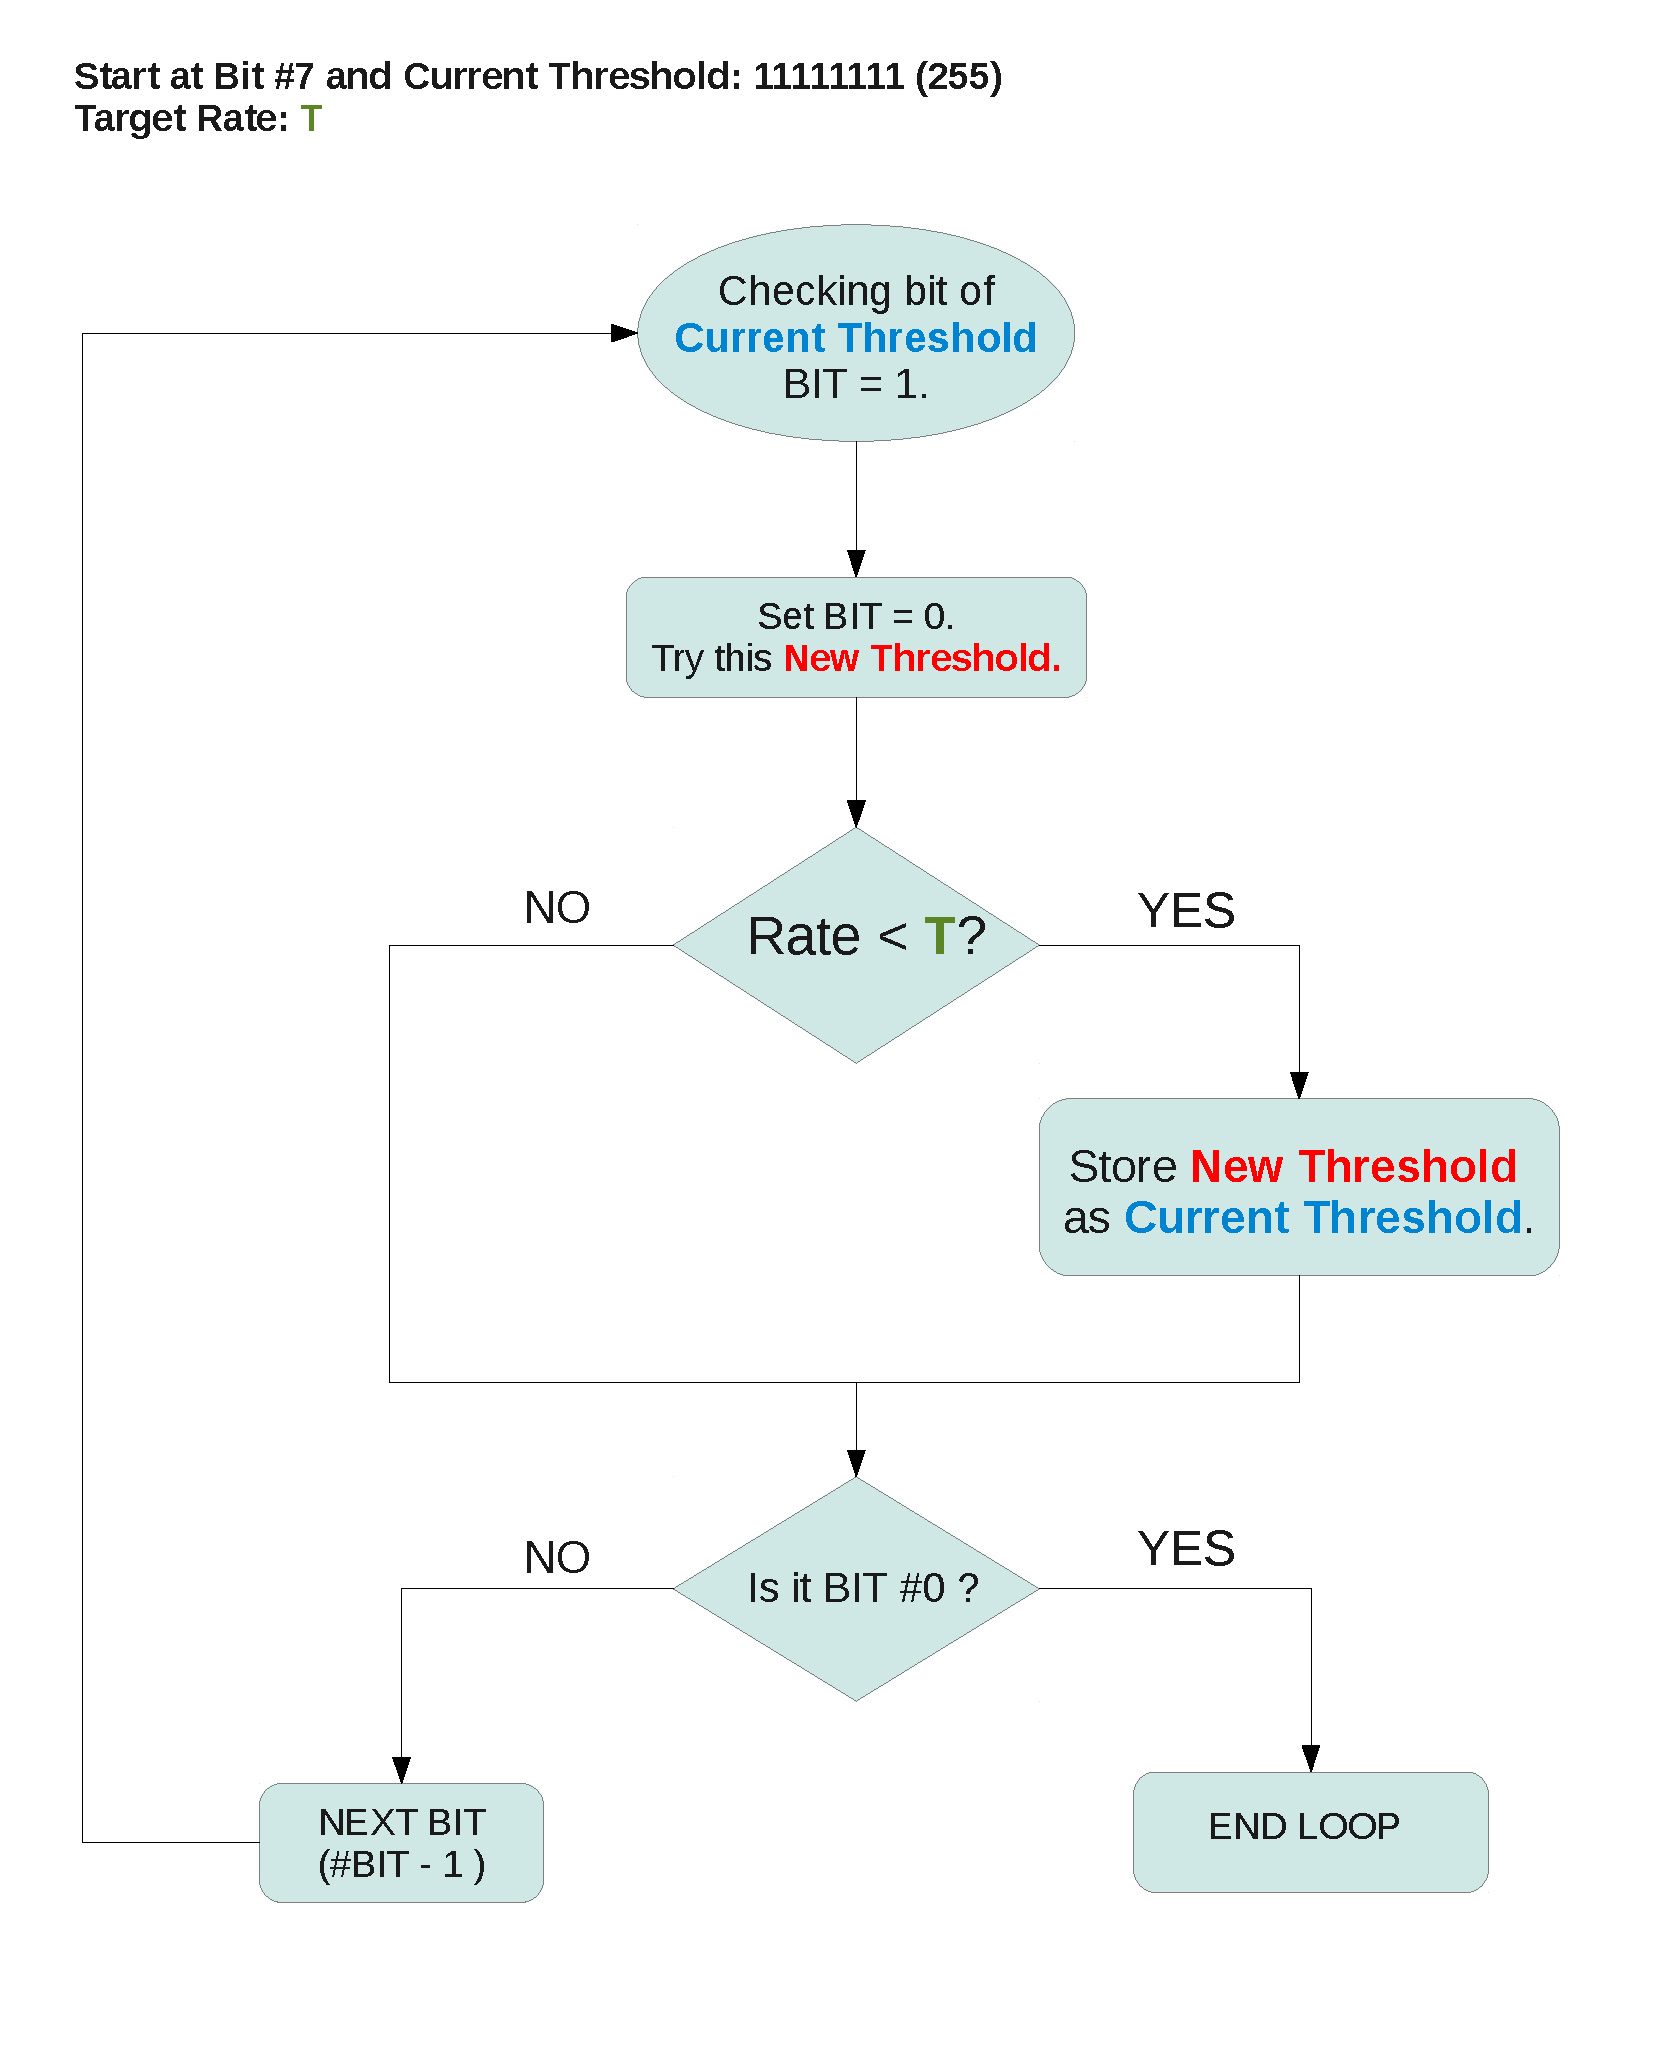
\includegraphics[width=0.7\textwidth]{./Pictures/calibrationalgorithm.pdf}
  \caption{Flux diagram of the calibration algorithm.}
  \label{fig:calalgorith}
\end{figure}

Once the loop is finished, the 50\% trigger rate threshold is calculated following the formula:

\begin{equation}
  50TH = \frac{(Target Rate-Baseline)}{(Baseline-Rate[Current Threshold-1]} + Current Threshold
\end{equation}

Being baseline the rate at the current threshold, say the last threshold that was stored in the loop.

\subsection{Calibration result}

When the full algorithm ends and runs over the 6 possible input signals, the obtained 50\% threshold can be plotted against the number of pixels added to see the calibration curve (see figure ~\ref{fig:calibcurve}).

\begin{figure}[h]
  \centering
  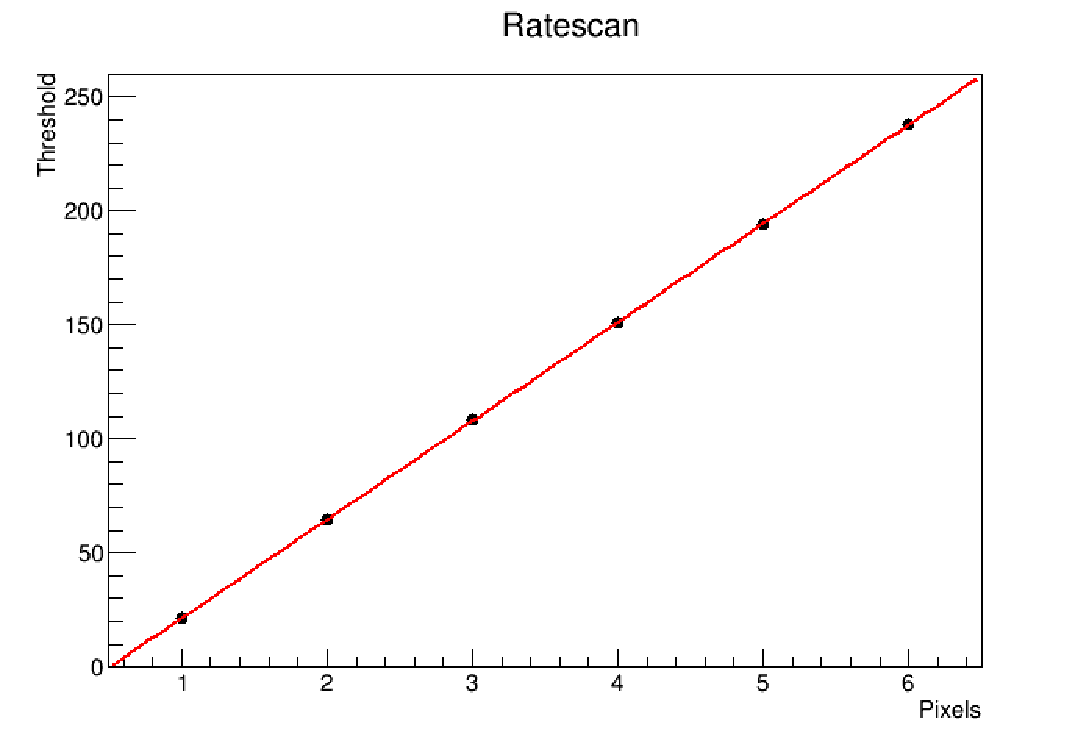
\includegraphics[width=0.7\textwidth]{./Pictures/calibcurve.pdf}
  \caption{Result of the rate scan for Adder A of one module.}
  \label{fig:calibcurve}
\end{figure}

If the initial pulse injected by the \gls{scb} is known and assuming that the adding is correct, the amplitude of each pulse is simply the multiplication of the initial pulse by the number of pixels added. This way, it is possible to obtain the gain and offset of the \gls{asic}.

\end{document}
